\documentclass{beamer}
\usepackage{ctex}
\usepackage{graphicx}
\usepackage{hyperref}
\usepackage{tikz}
\usetikzlibrary{shapes.geometric, arrows}
\usepackage{pgf-pie}

\makeatletter
\def\input@path{{../styles}}  % 
\makeatother
\usepackage{ubeamer}
\uBigPaper

\title{中学生学习C++程序设计的优势}

\begin{document}

\frame{\titlepage}
\begin{frame}[t]{万物皆可算,处处是程序}
\begin{columns}
\column{0.9\textwidth}
\begin{spacing}{1.1}
\large
\begin{enumerate}[label={\arabic*.}]
\item 操作系统:Windows,macOS,iOS,Android
\item 办公软件:LaTeX,Word,Excel,PowerPoint
\item 智能手机应用:微信、QQ、淘宝、抖音、地图
\item 网站:任何网站
\item 汽车:智能驾驶,车载娱乐系统
\item 医疗设备:医疗成像系统(如CT、MRI)
\item 娱乐与游戏:手机游戏、爱奇艺、腾讯视频
\item 金融与电子支付:支付宝、银行App,股票交易、期货交易
\item 物联网(IoT)设备:智能家居设备、机器人、无人机
\item 人工智能:DeepSeek,ChatGPT,豆包、Kimi
\end{enumerate}
\end{spacing}
\end{columns}
\end{frame}

\begin{frame}[t]{什么是程序设计}
程序设计是指根据特定需求,通过一系列的\alert{逻辑思考、分析、规划和编写代码},最终实现功能的过程。它不仅仅是写代码那么简单,还包括了从问题的定义、解决方案的设计、实现方式的选择,到最终的调试、优化和维护的全过程。\\
\vspace*{1cm}
简单来说,程序设计就是\alert{将一个具体问题转化为计算机能够理解和执行的步骤},并通过编程语言进行表达的过程。
\end{frame}

% 全球编程语言平均薪资
\begin{frame}{全球程序设计语言平均薪资排名}
\begin{columns}
\column{0.9\textwidth}
\begin{spacing}{1.5}
\Large
    \begin{enumerate}[label={\arabic*.}]
        \item C++: 12万美元
        \item Java: 11万美元
        \item Python: 10.5万美元
        \item C: 10万美元
        \item JavaScript: 9.5万美元
    \end{enumerate}
\end{spacing}
\end{columns}
\end{frame}

% 全球编程语言使用人数
\begin{frame}{全球主要程序设计语言使用人数占比}
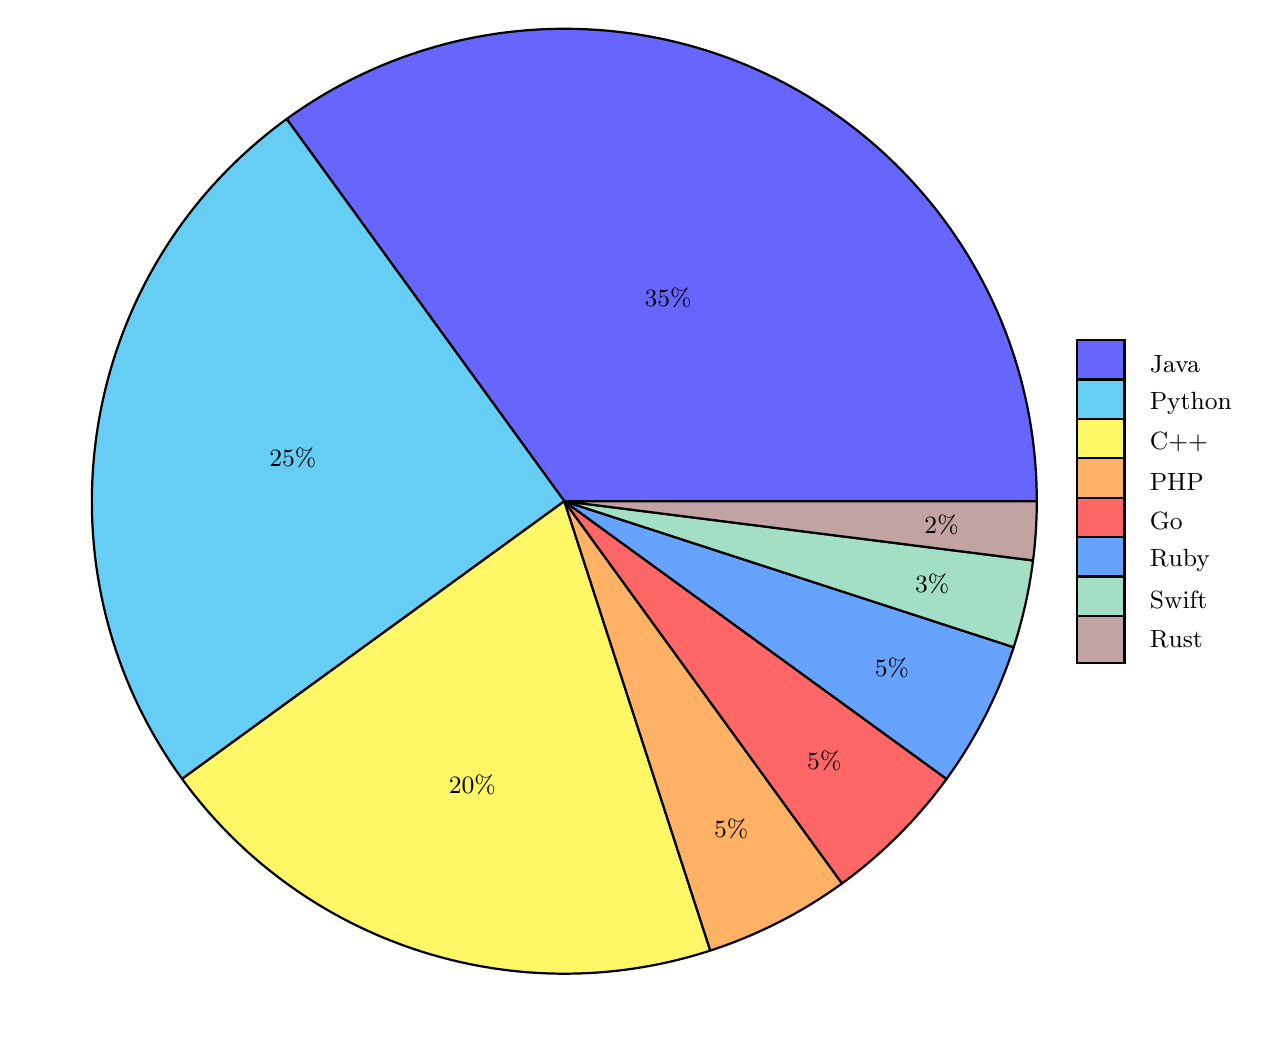
\begin{tikzpicture}[scale=2]
    \pie[radius=3, text=legend, align=left, font=\small, nodes={inner sep=3mm}]{
        35/Java,
        25/Python,
        20/C++,    
        5/PHP,
        5/Go,
        5/Ruby,
        3/Swift,
        2/Rust
    }
\end{tikzpicture}
\end{frame}

\begin{frame}[t]{C++语言的特点}
\begin{columns}
\column{0.9\textwidth}
\begin{spacing}{1.2}
\large
    \begin{enumerate}[label={\arabic*.}]
    \item C++是一种编译型语言,能够直接与硬件交互,因此执行速度非常快,适合高性能计算和需要低延迟的应用。例如,游戏引擎、操作系统、嵌入式系统等领域。
	\item 适合需要高性能、系统级编程的应用,如游戏开发、操作系统、嵌入式系统、图形渲染、金融领域等。C++对于低级硬件控制和优化是不可或缺的。\\
	\item C++语法严谨,适合作为第一门程序设计语言学习,有助于培养学习者培养严谨的编程习惯。C++的用户更容易学习其它程序设计语言。
    \end{enumerate}
\end{spacing}
\end{columns}
\end{frame}

% 全球五大学科竞赛
\begin{frame}{全球五大学科竞赛}

\begin{columns}
\column{0.9\textwidth}
\begin{spacing}{1.2}
\large
竞赛名称及年份:\\
\begin{enumerate}[label={\arabic*.}]
    \item 数学奥林匹克(Mathematical Olympiad: IMO):1959年,罗马尼亚
    \item 物理奥林匹克(Physics Olympiad: IPhO)1967年,匈牙利
    \item 化学奥林匹克(Chemistry Olympiad: IChO):1968年,捷克斯洛伐克
    \item 生物奥林匹克(Biology Olympiad: IBO):1970年,德国
    \item 信息学奥林匹克(Informatics Olympiad: IOI):1989年,匈牙利
\end{enumerate}
\end{spacing}
\end{columns}
\end{frame}

% 时间轴展示
\begin{frame}{信息学主要竞赛与认证}
    \begin{tikzpicture}[xscale=1.2, yscale=1.2]
    \draw[orange, ->, >=stealth, line width=0.2cm] (0,0) -- (24,0);    
    \fill  (4,0) [red] circle(0.3cm) node [rectangle, fill=blue!20, text width=6cm, align=center, below=1cm]  {1984\\NOI\\全国信息学奥林匹克竞赛};    
    \fill  (8,0) [blue] circle(0.3cm) node [rectangle, fill=blue!20, text width=6cm, align=center, above=1cm]  {1989\\IOI\\国际信息学奥林匹克竞赛};
    \fill  (12,0) [red] circle(0.3cm) node [rectangle, fill=blue!20, text width=6cm, align=center, below=1cm] {2003\\APIO\\亚太地区信息学奥林匹克竞赛};    
    \fill  (16,0) [blue] circle(0.3cm) node [rectangle, fill=blue!20, text width=6cm, align=center, above=1cm] {2006\\NOIP\\全国青少年信息学奥林匹克联赛};
    \fill  (20,0) [red] circle(0.3cm) node [rectangle, fill=blue!20, text width=6cm, align=center, below=1cm] {2010\\CSP\\计算机科学能力认证};    
    \end{tikzpicture}
    
	\begin{enumerate}[label={\arabic*.}]
    \item CSP:计算机软件能力认证
    \item NOIP:全国青少年信息学奥林匹克联赛
    \item NOI:全国信息学奥林匹克竞赛
    \item APIO:亚太地区信息学奥林匹克竞赛
    \item IOI:国际信息学奥林匹克竞赛
    \end{enumerate}
\end{frame}

% 参加NOI竞赛的好处
\begin{frame}[t]{参加NOI竞赛的好处}
\begin{columns}
\column{0.9\textwidth}
\begin{spacing}{1.2}
\large
    \begin{enumerate}[label={\arabic*.}]
	\item NOI金牌前50名可保送至清华大学、北京大学
	\begin{itemize}
		\item 51~60名金牌: 强基计划破格资格+985高校签约
        \item 银牌: 36所强基高校破格入围
        \item 铜牌: 综合评价招生重要筹码
    \end{itemize}
    \item 激发对计算机科学的兴趣
    \item 增强逻辑思维和问题解决能力
    \item 提高学习的自主性,培养自学能力
    \item 提前认知学科与专业,为未来的学术和职业生涯打下坚实的基础
    \end{enumerate}
\end{spacing} 
\end{columns}
\end{frame}

% 学习C++编程的好处
\begin{frame}{学习C++编程的好处}
\begin{columns}
\column{0.9\textwidth}
\begin{spacing}{1.2}
\large
    \begin{itemize}
        \item 提高逻辑思维与问题解决能力
        \item 培养严谨的思维方式和编程规范
        \item 加强对计算机硬件与软件原理的理解
        \item 对其他编程语言(如Python、Java)的学习起到铺垫作用
        \item 开阔眼界,提升全球竞争力
    \end{itemize}
\end{spacing} 
\end{columns}
\end{frame}

% 学习C++对孩子学业的帮助
\begin{frame}{学习C++程序设计对学业的帮助}
\begin{columns}
\column{0.9\textwidth}
\begin{spacing}{1.2}
\large
    \begin{itemize}
        \item 锻炼抽象思维与数学建模能力
        \item 增强自学能力与独立思考能力
        \item 提高理工科领域的学术竞争力
        \item 培养团队合作与解决复杂问题的能力
        \item 打开通往计算机科学、电子工程等领域的大门
    \end{itemize}
\end{spacing} 
\end{columns}
\end{frame}

\begin{frame}[t]{晋城市学习C++程序设计参加NOIP及NOI竞赛的案例}
\begin{columns}
\column{0.9\textwidth}
\begin{spacing}{1.4}
\normalsize
    \begin{enumerate}[label={\arabic*.}]
    \item 赵赟峰,2014年NOIP一等奖,2015年获第32届全国青少年信息学奥林匹克竞赛金牌,2016年保送清华大学
	\item 甄子豪,2017年获NOIP一等奖,2018年获NOIP一等奖,2019年获第36届全国青少年信息学奥林匹克竞赛金牌,2020年保送清华大学
	\item 丁子尧,2017年获NOIP一等奖,2018年获NOIP一等奖,2019年获第36届全国青少年信息学奥林匹克竞赛铜牌,2020年以高考成绩666分考入中国科学技术大学
	\item 董凯文,2017年NOIP一等奖,2018年NOIP一等奖,2019年获第36届全国青少年信息学奥林匹克竞赛铜牌,2020年以高考成绩650分考入北京邮电大学
\end{enumerate}
\end{spacing} 
\end{columns}
\end{frame}

\begin{frame}[t]{模拟考试成绩与高考成绩}
\vspace*{1cm}
\centering
\begin{spacing}{1.5}
\large
2019年7月27日参加第三次模拟考试,2020年7月7日参加高考。\\
\vspace{2cm}
\begin{tabular}{|c|c|c|c|c|c|c|c|c|}
\hline
科目 & 语文 & 数学 & 英语 & 物理 & 化学 & 生物 & 理综 & 总分 \\
\hline
三模 & 86 & 118 & 109 & 66 & 56 & 63 & 185 & 498 \\
\hline
高考 & 121 & 140 & 129 &  &  &  & 276 &  666\\
\hline
\end{tabular}
\end{spacing}
\end{frame}

\begin{frame}[t]{NOI经历对大学学习的巨大帮助(丁子尧)}
\begin{columns}
\column{0.95\textwidth}
\begin{spacing}{1.1}
\large
    \begin{enumerate}[label={\arabic*.}]
    \item 2021年11月,获第7届中国大学生程序设计竞赛威海站银牌
	\item 2021年11月,获第46届国际大学生程序设计竞赛济南站金牌
	\item 2021年12月,获第46届国际大学生程序设计竞赛南京站银牌
	\item 2022年7月,获第46届国际大学生程序设计竞赛亚洲区决赛银牌
	\item 2022年10月,获第47届国际大学生程序设计竞赛西安站金牌
	\item 2022年11月,获第47届国际大学生程序设计竞赛沈阳站金牌
	\item 2023年3月,获第47届国际大学生程序设计竞赛亚洲区决赛铜牌
	\item 2023年10月,获优秀应届本科毕业生免试攻读硕士研究生资格
	\item 2024年4月,参加第47届国际大学生程序设计竞赛全球总决赛
	\item 2024年至今,中国科学技术大学攻读硕士学位
\end{enumerate}
\end{spacing} 
\end{columns}
\end{frame}

\begin{frame}[t]{终身学习}
\begin{columns}
\column{0.95\textwidth}
\begin{spacing}{1.1}
\large
    \begin{enumerate}[label={\arabic*.}]
    \item 自主学习的兴趣
	\item 自主设置的目标
	\item 自主学习的方法
	\item 匹配的路径资源
\end{enumerate}
\end{spacing} 
\end{columns}
\end{frame}

\begin{frame}[t]{致谢}
\large
\centering
\vspace*{4cm}
特别感谢牛校长、杨校长与各位领导和老师的大力支持!\\
\vspace*{1cm}
诚挚感谢在座嘉宾与家长的到场、持续关注与耐心聆听!\\
\vspace*{1cm}
祝愿孩子们早日插上人工智能的翅膀,扶摇直上九万里!
\end{frame}

\begin{frame}[t]{会后交流}
微信面对面建群:\\
\begin{itemize}
    \item 右上角\textcircled{+}
    \item 发起群聊
    \item 面对面建群
    \item 输入数字:\alert{2025}
    \item 进入该群
    \end{itemize}
\end{frame}

\end{document}
